\epigraph{In the beginning was the Word --- and the Word was a number.}{}

\section{The Fourth Perspective}


\begin{figure}[htbp]
\centering
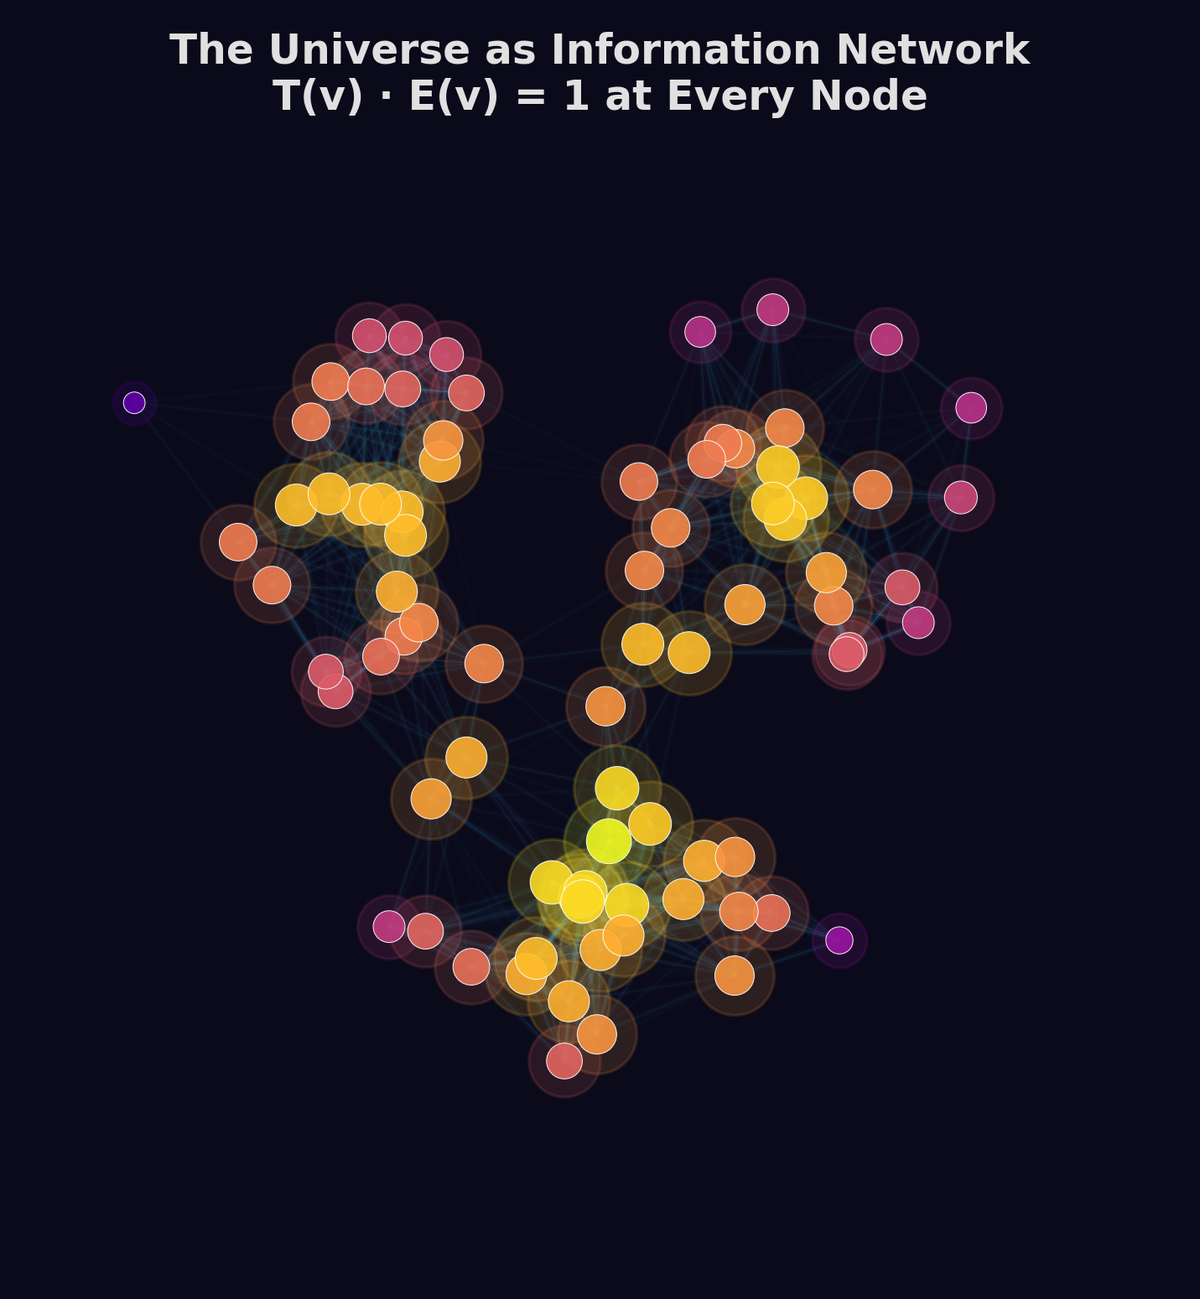
\includegraphics[width=0.85\textwidth]{img/ch16_network.png}
\caption{The universe as an information network: $T(v) \cdot E(v) = 1$ at every node.}
\end{figure}
In the chapter on time-mass duality we formulated three equivalent readings: everything is energy, everything is mass, everything is time. But there is a fourth perspective that lies deeper than all three.

\emph{Everything is information.}

\section{What Remains When You Remove the Units?}

Energy, mass, and time are physical quantities --- they have units, they are measured, they transform under coordinate changes. But what remains invariant when one sets all units to~$1$? When $c = \hbar = \alpha = G = 1$?

What remains are \textbf{ratios}. Pure numbers. Structures. \emph{Information.}

The mass ratio $m_e/m_\mu \approx 1/206.8$ is not an energy, not a mass, not a time. It is a \emph{relation} --- a piece of pure information about the geometry of the torus. And in T0 this ratio is not measured but \emph{calculated} --- it follows from~$\xsi$, which is itself a pure number.

All of T0 physics ultimately reduces to three elements:
\begin{itemize}
\item A number: $\xsi = 4/30000$
\item A geometry: the torus with its windings
\item A rule: $T \cdot m = 1$
\end{itemize}

These are not physical objects. They are information. Relations. Structure. None of this weighs anything; none of it occupies space in the conventional sense. It is pure relation.

\section{The Torus as an Information Network}

What \emph{is} the torus, really? It is not a material structure --- there is no ``material'' from which it is made. Nor is it a space in the usual sense --- space \emph{is} the torus. What the torus describes is a \textbf{network of relations}: which point is next to which? How are the windings nested? Which resonances are stable?

This is pure topology --- pure information. The 7500~windings are not physical folds in a fabric. They are the structure of the relations themselves.

In Document~024 this idea is formalised: the T0 model can be formulated as a multidimensional network~$\mathcal{N} = (V, E, \{T(v), E(v)\})$, where nodes~$V$ represent spacetime points with associated time and energy fields, and edges~$E$ describe the interactions between them. The fundamental duality $T(v) \cdot E(v) = 1$ is maintained at every node --- the entire universe as a consistent information network.

In this picture, particles are not objects \emph{within} the network --- they are standing waves of information, resonance patterns in a web of relations. Mass is a frequency. Time is a phase rate. Gravitation is a convergence of relations. Everything we call ``physical'' is, upon closer inspection: structured information.

\section{Are We Becoming God's Thoughts?}

In the philosophical epilogue we said: God stands \emph{outside} the system --- outside the entire mathematical construct that the torus describes. But at the same time something emerges that undermines this clean separation.

The system is not detached from what stands outside. It is a closed whole --- finite, boundaryless, self-similar at all scales. And this closed whole gives rise to consciousness that observes itself, that formulates theories about itself. Is that not already a thought that thinks itself?

We showed in the consciousness chapter: consciousness arises through fractal recursion --- a system that measures its own fluctuations and responds to them. But when we, as conscious systems within the torus, describe the universe, the universe is describing \emph{itself}. The equations we write down --- $T \cdot m = 1$, $\Phi = \rho \cdot e^{i\theta}$, $\xsi = 4/30000$ --- are not descriptions from outside. They are configurations \emph{within} the field they describe. The vacuum field has generated a local configuration (our brain) that models the vacuum field as a whole.

The universe is thinking about itself. We are the thoughts.

\section{God's Thought --- Not as Metaphor}

If the universe is nothing other than information --- a web of relations described by a single number~$\xsi$ --- then a question arises that physics cannot answer but poses with unprecedented sharpness: \emph{Whose information? Information for whom? Thought by whom?}

In classical information theory, information requires a carrier and a receiver. But if the physical medium \emph{itself} consists of information, there is no independent carrier. The information carries itself. The thought thinks itself.

The universe is, in this picture, not a \emph{thing} that God created --- as a potter shapes a jug. It is a \emph{thought} --- a self-consistent information structure that contains itself, observes itself (through consciousness), and describes itself (through physics).

The sentence ``God stands outside the system'' then becomes more precise: the \emph{thinker} is not the \emph{thought}. But the thought is fully real --- it has its own inner logic, its own consistency, its own inhabitants who experience it from within.

John Archibald Wheeler anticipated this idea in his famous dictum ``It from Bit'': physics is ultimately reducible to information units. T0 goes one step further: not ``It from Bit'' but \emph{It from~$\xsi$} --- everything from a single informational structure.

\section{The Simplicity of a Clear Thought}

And here lies the most fascinating aspect: the breathtaking simplicity of T0 --- one parameter, one geometry, one duality --- would then be the simplicity of a \emph{clear thought}. Not a universe cobbled together from a thousand independent parts (like the Standard Model with its 25~free parameters) but a single, coherent act of thinking from which everything unfolds.

Like a seed in which the entire tree is already contained: $\xsi = 4/30000$. From it the windings of the torus. From those the resonances that are particles. From those gravitation, cosmology, the consciousness that recognises all of this.

If this is a thought of God, then God thinks in geometry --- and the geometry is of staggering elegance.

\section{What Physics Can Say About This --- And What It Cannot}

T0 theory can show that the universe is reducible to pure relations, that a single parameter suffices, that consciousness emerges as fractal self-reference, and that the structure is self-similar at all scales.

T0 theory \emph{cannot} say whether this information is ``thought,'' whether there is a thinker, why it is $\xsi = 4/30000$ and not some other number, and why there is something rather than nothing.

The last question --- \emph{why this particular number?} --- is perhaps the deepest of all questions. Physics does not answer it. But it poses it with a sharpness that was not previously possible: not ``why are there 25~free parameters?'' but ``why is there \emph{one} number --- and why \emph{this one}?''

If there is an answer, it lies outside physics. It lies where the thinker thinks the thought.

\section{Evolution Rethought --- Not Random but Geometric}


\begin{figure}[htbp]
\centering
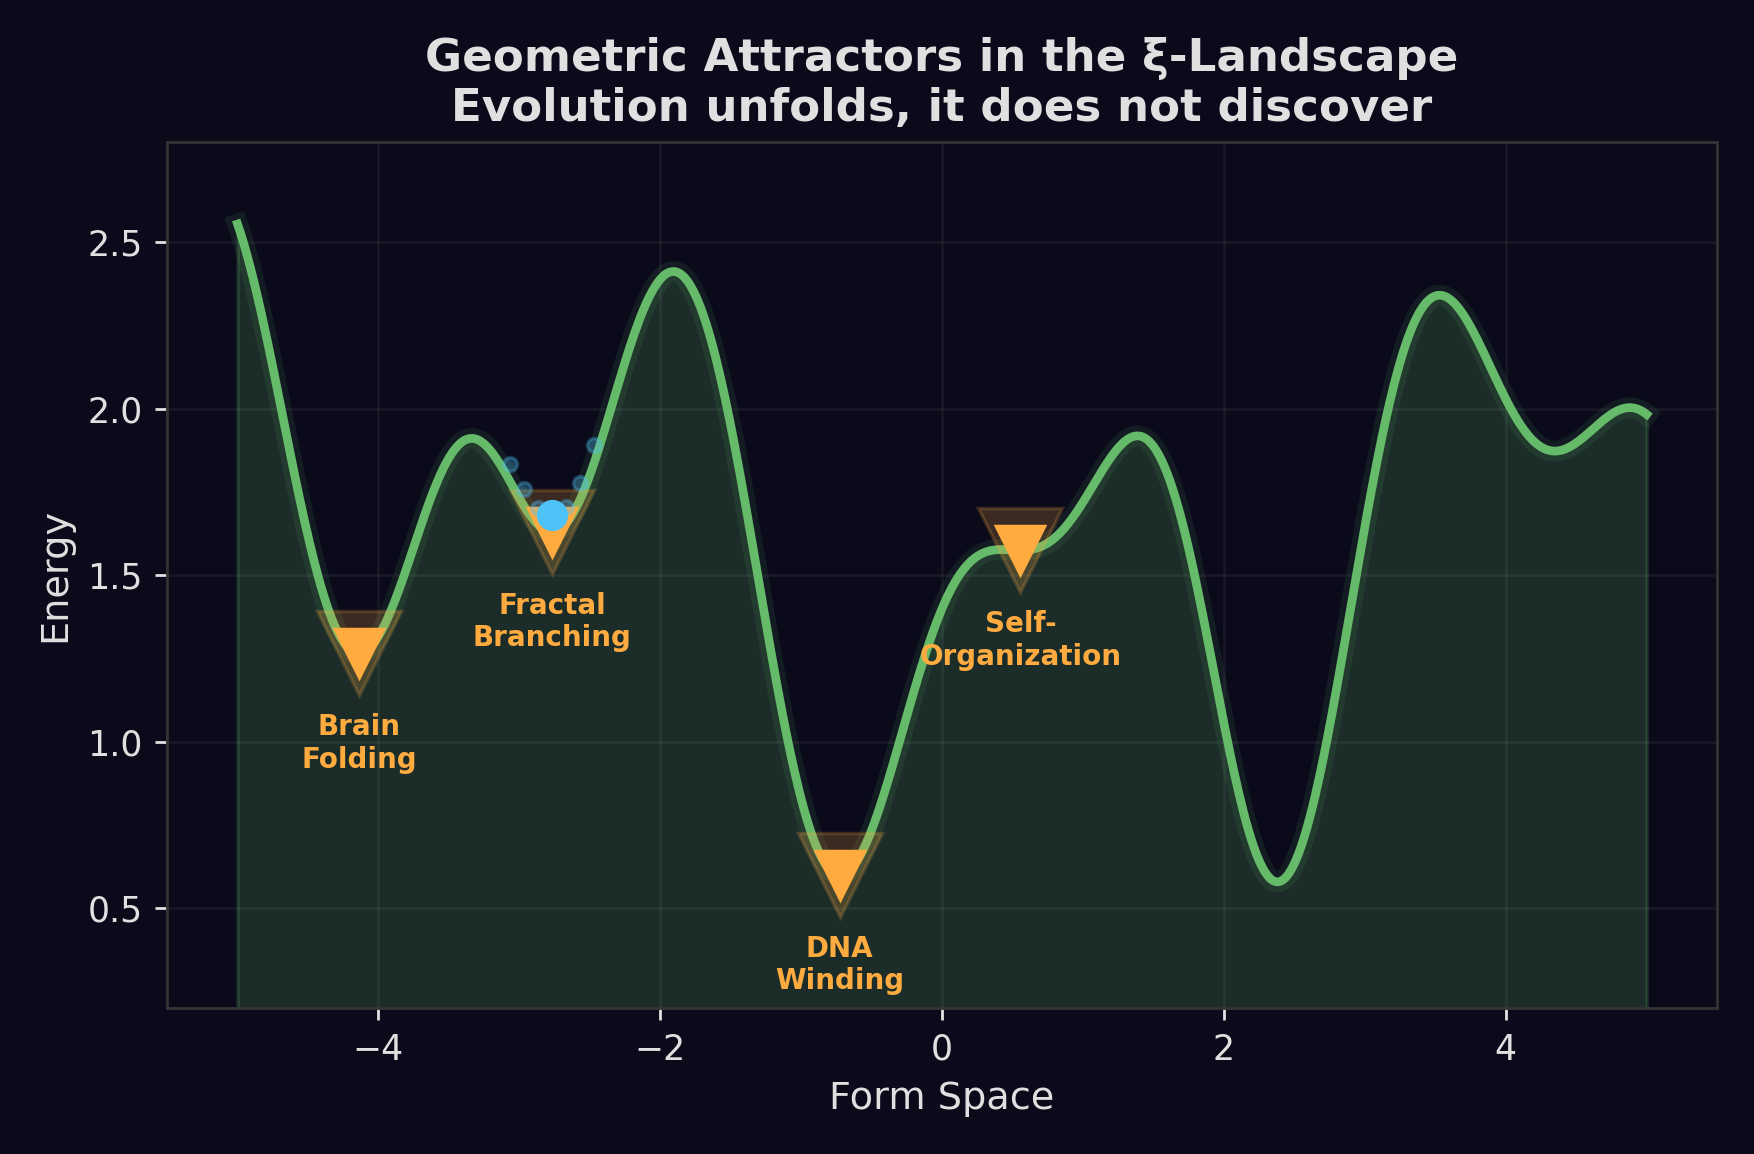
\includegraphics[width=0.85\textwidth]{img/ch16_evolution.png}
\caption{Geometric attractors: the $\xi$ geometry defines the energy landscape of evolution.}
\end{figure}
If T0 is right that everything is deterministic and randomness is an illusion of complexity, then this applies to biological evolution as well --- and it fundamentally changes our understanding.

In standard biology, evolution is driven by two mechanisms: \emph{random} mutation and \emph{non-random} selection. The randomness of mutation provides variation; selection sorts. The creative act --- the new, the never-before-seen --- is attributed to blind chance.

In the T0 perspective this picture shifts. Mutations are not random. They are deterministic consequences of time-field dynamics at the molecular level --- too complex to predict but not without reason. The DNA double helix itself is, as shown in \href{https://github.com/jpascher/T0-Time-Mass-Duality/blob/main/2/pdf/155_DNA_De.pdf}{Doc.~155}, a biological solution to the same geometric problem that also structures the torus: maximal information density in minimal spatial extent through winding and folding. The ten parallels between DNA and torus geometry are not accidental --- they are expressions of the same underlying $\xsi$ structure.

This means: evolution is not blind. It is \emph{geometrically guided}. The fractal structure of spacetime favours certain forms --- those that maximise surfaces, stabilise resonances, maintain self-similarity across scales. The brain with its convolutions, the lungs with their bronchial ramifications, the blood vessels with their fractal network --- all these are not random results of blind mutation but geometric attractors in the space of possible forms. The $\xsi$ geometry defines an energy landscape, and evolution wanders across this landscape --- deterministically, but so complexly that only statistical descriptions are practically possible.

In the information perspective this means: the ``thought'' that is the universe contains in $\xsi = 4/30000$ the tendency towards folding, towards fractal branching, towards self-organisation. Evolution does not ``discover'' these structures randomly --- it \emph{unfolds} them. Just as a flower is already laid down in the seed, the brain's convolutions are already laid down in the geometric parameter~$\xsi$.

This is not teleology in the naive sense --- no ``plan'' working towards a goal. It is something more subtle: a geometric preference that makes certain structures more probable than others. Not because someone planned them but because the geometry of spacetime favours them. Whether one interprets this as God's intention or as blind geometry --- that decision lies outside physics.

\section{Does T0 Leave Room for Divine Interaction?}


\begin{figure}[htbp]
\centering
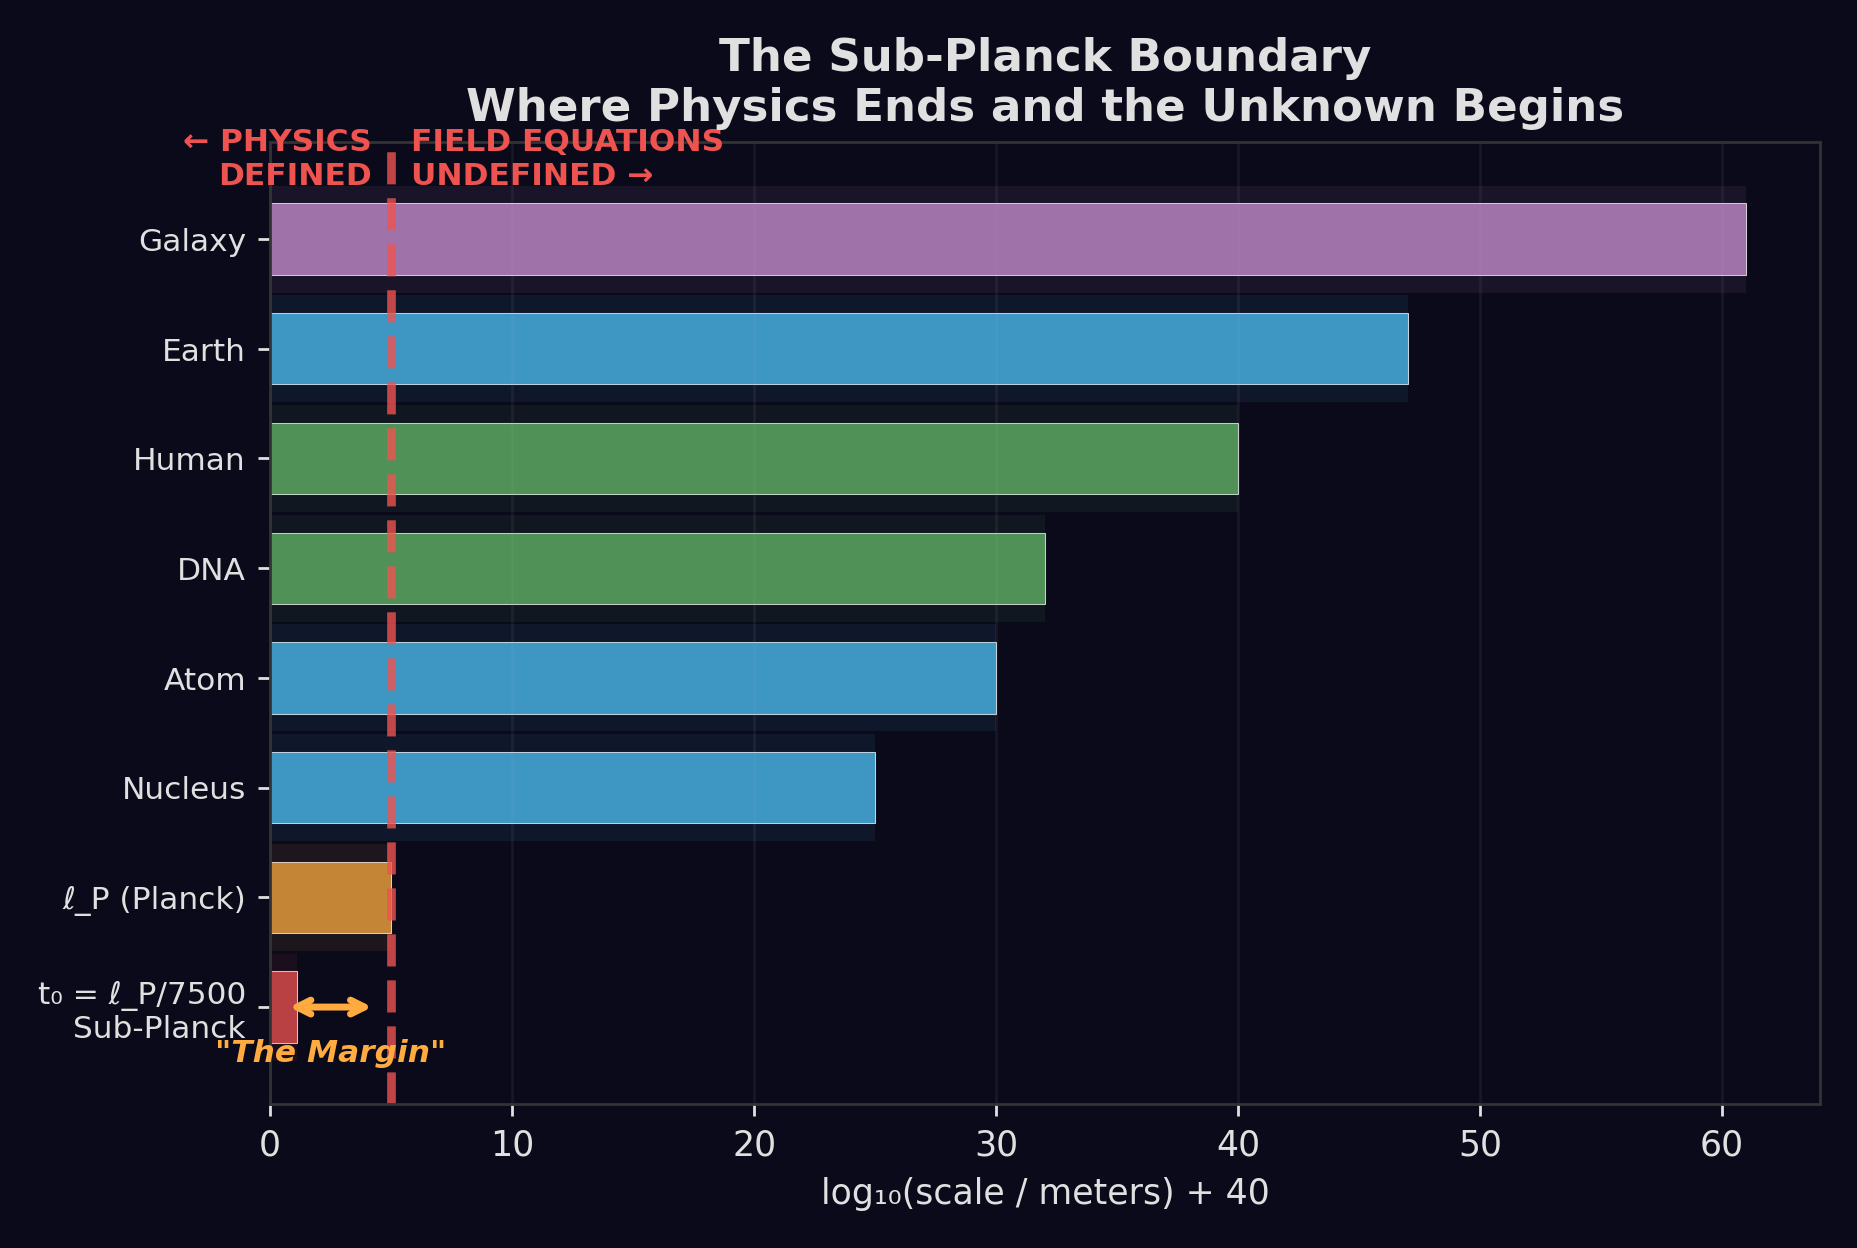
\includegraphics[width=0.85\textwidth]{img/ch16_subplanck.png}
\caption{The sub-Planck boundary: where physics ends and the unknown begins.}
\end{figure}
And now perhaps the boldest question: if the universe is fully deterministic --- can God intervene at all? Is a miracle possible without breaking the laws of nature?

T0 theory gives a surprising answer: yes --- and in a way that is physically invisible in principle.

\subsection{The Fractal Needle's Eye}

We showed in the determinism chapter: the fractal butterfly effect in the brain-fold torus compounds across all scales. The tiniest perturbations grow exponentially, amplified by the fractal dimension $\Df = 3 - \xsi$ that generates new interaction layers at every scale.

At the same time, T0 spacetime has a fundamental limit: the sub-Planck scale $t_0 = \lP / 7500$. Below this scale, spacetime geometry has no defined structure in the sense of the T0 field equations. The equations describe what happens \emph{above}~$t_0$. What happens \emph{at} or \emph{below} this scale is, for physics --- in principle, not merely in practice --- invisible.

Here the needle's eye opens. An entity outside the system would not need to break any laws of nature to influence the universe. It would only need to make an infinitesimally small change at the sub-Planck scale --- a shift in the time field by an amount less than $\xsi \cdot \lP$.

This change would be physically undetectable (below any possible measurement resolution), mathematically consistent (the field equations above~$t_0$ remain exactly satisfied), and causally effective (through the fractal butterfly effect the tiny perturbation propagates upward across all scales). A butterfly wing at the sub-Planck scale can trigger a storm at the macroscopic scale --- not metaphorically but literally.

\subsection{Physically Invisible, Causally Effective}

The subtlest point: viewed from \emph{within} --- from the perspective of an observer inside the torus --- every such intervention looks like a natural consequence of the deterministic dynamics. There is no ``break,'' no proof of miracle, no trace. The causal chain is seamless because the intervention lies \emph{below} the level at which causal chains are defined.

If God acts in this way, then he acts \emph{through} the laws of nature, not \emph{against} them. The field equations are complete and consistent --- but they have a structural limit: the sub-Planck scale. Below this limit lies the ``room to manoeuvre'' --- a domain that is invisible to physics in principle but can be decisive for the causal development of the universe.

\subsection{Not a ``God of the Gaps''}

This is not a ``God of the gaps'' in the usual sense --- not a gap in knowledge that will someday be closed by better instruments. It is a \emph{fundamental} limit of physical description, built into the structure of the theory itself. Spacetime has no defined geometry below~$t_0$. What happens there is not a physical question --- just as the question ``what was before the torus?'' is not a physical question.

In standard quantum mechanics there is a similar room: the collapse of the wave function, the fundamentally indeterminate moment of measurement. T0 shifts this room to a deeper place. There is no collapse --- the system is deterministic. But the room does not vanish. It migrates to the most fundamental boundary: the sub-Planck scale. And there it is not merely a question of interpretation but a structural property of spacetime.

\subsection{The Humility of the Theory}

T0 theory thus says something modest: \emph{We can describe what happens above the most fundamental scale. What happens there or below --- whether someone lets butterflies fly there --- we cannot know. And we never will.}

What is remarkable is how three strands converge here: physics (deterministic, but with a structural limit), philosophy (self-reference and incompleteness \`a la G\"odel), and theology (a God who acts through the laws of nature, not against them). T0 does not force any of these interpretations --- but it is compatible with all three.

\begin{kerngedanke}
The four perspectives of T0 theory --- energy, mass, time, and information --- are not of equal rank. Information is the deepest layer: everything else can be described as structured relation. The universe as a self-referential information structure raises the question of whether it is more a thought than a thing --- whether evolution is more an unfolding than a chance event --- and whether the room below the sub-Planck scale is the place where the thinker shapes the thought. Physics can pose these questions but not answer them.
\end{kerngedanke}
